\documentclass{article}
\usepackage{graphicx} % Required for inserting images
\usepackage{geometry}
\usepackage{circuitikz}
\usepackage{siunitx}
\usepackage{CJKutf8}
\usepackage{amsmath}
\usepackage{amssymb}
\usepackage{caption}
\usepackage{float}
\usepackage{subcaption}
\geometry{top=10mm, left=20mm, a4paper}




\title{MOS-Based Differential Circuits Report}
\author{梁程捷 (B11901136), 吳奕娃 (B11901080)}
\date{}


\begin{document}
\begin{CJK*}{UTF8}{bkai}
\maketitle
%========DC Analysis=================
\section{DC Analysis}
\begin{equation*}
    I_1 = 0.129 \text{ \unit{\milli\ampere}}, \, I_2 = 0.156 \text{ \unit{\milli\ampere}}, \, I = 0.280 \text{ \unit{\milli\ampere}}
\end{equation*}
\textbf{$I_1 \ne I_2$} due to mismatch in circuit components and transistor parameters.\\
\textbf{$I_1 + I_2 = I$} because of \textit{Kirchhoff's Current Law}.\\

%=========AC Analysis=================
\section{AC Analysis}

For $f$ = 1 \unit{\kilo\hertz}, $V_i(V_{pp})$ = 0.9 \unit{\volt}, $V_{od}(V_{pp})$ = 1.8 \unit{\volt}, \underline{\textbf{$A_d$ = 2 \unit{\volt}/\unit{\volt}}}. \\

\begin{figure}[h]
    \begin{center}
    \begin{subfigure}[b]{0.40\textwidth}
        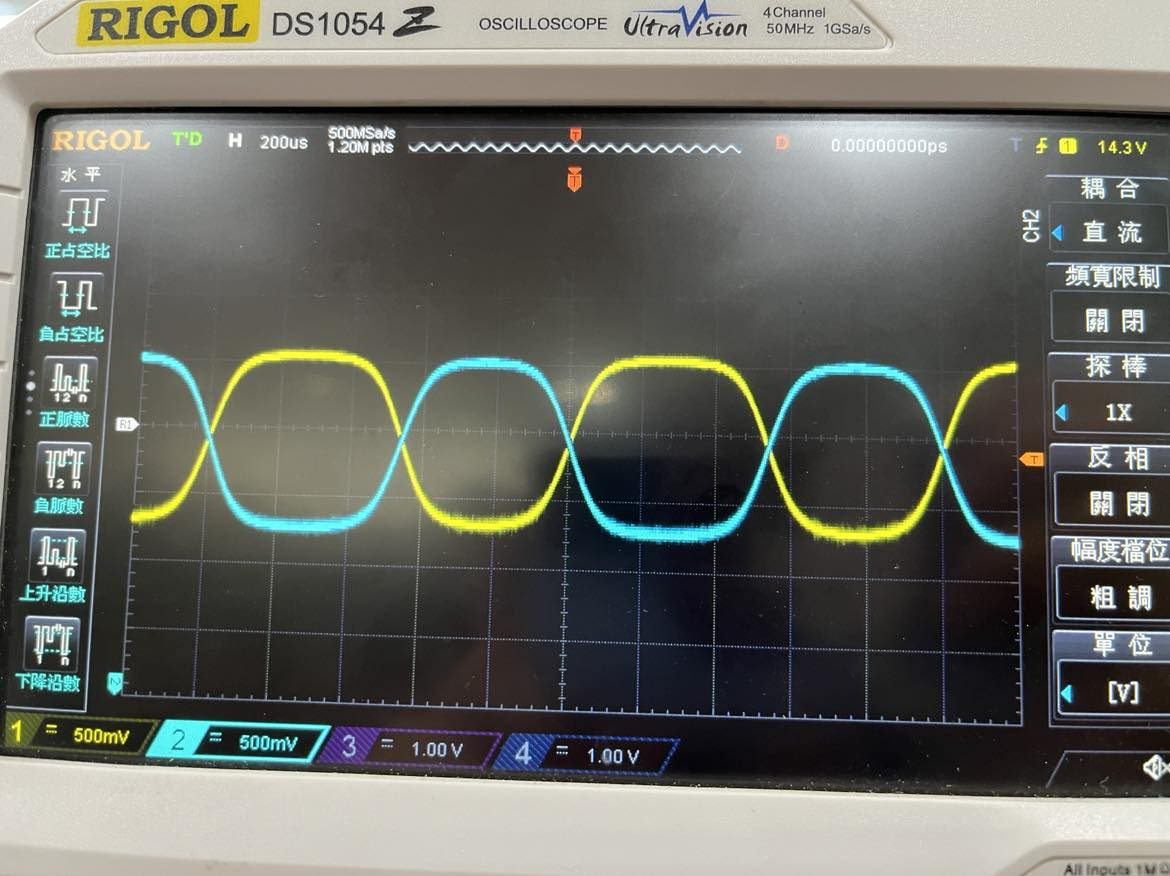
\includegraphics[width=\textwidth]{Vo1_and_Vo2.jpg}
        \caption*{Waveforms of $V_{o1}$ (CH1) and $V_{o2}$ (CH2)}
    \end{subfigure}
    ~
    \begin{subfigure}[b]{0.40\textwidth}
        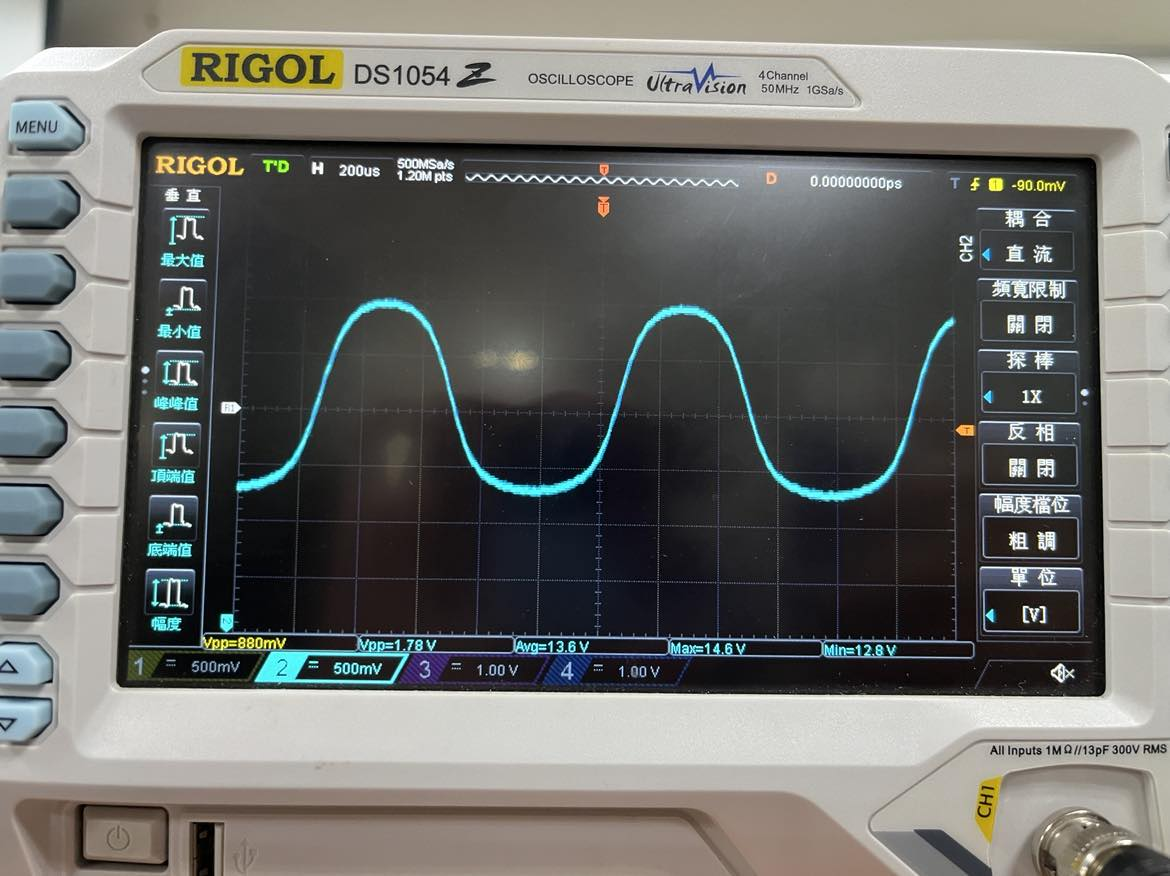
\includegraphics[width=\textwidth]{Vod.jpg}
        \caption*{Waveform of $V_{od}$}
    \end{subfigure}
\end{center}
\end{figure}


\begin{minipage}{0.5\textwidth}
\begin{table}[H]
    \begin{tabular}{|c|c|c||c|c|c|}
        \hline
        $f$ (\unit{\kilo\hertz}) &  $V_i$ (V)& $V_{od}$ (V) & $f$ (\unit{\kilo\hertz}) &  $V_i$ (V)& $V_{od}$ (V)\\
        \hline\hline
            1   & 0.9  & 1.8  & 100 & 0.88 & 1.72 \\
            5   & 0.88 & 1.8  & 150 & 0.88 & 1.62 \\
            10  & 0.88 & 1.78 & 200 & 0.88 & 1.52 \\
            20  & 0.88 & 1.78 & 250 & 0.88 & 1.42 \\
            30  & 0.88 & 1.78 & 300 & 0.88 & 1.3  \\
            50  & 0.88 & 1.76 & 330 & 0.88 & 1.24 \\
            80  & 0.88 & 1.74 & 350 & 0.86 & 1.2  \\
        \hline
    \end{tabular}
    \caption{AC analysis raw experimental data}
\end{table}
\end{minipage}\hspace{20mm}
\begin{minipage}{0.5\textwidth}
    \begin{figure}[H]   
        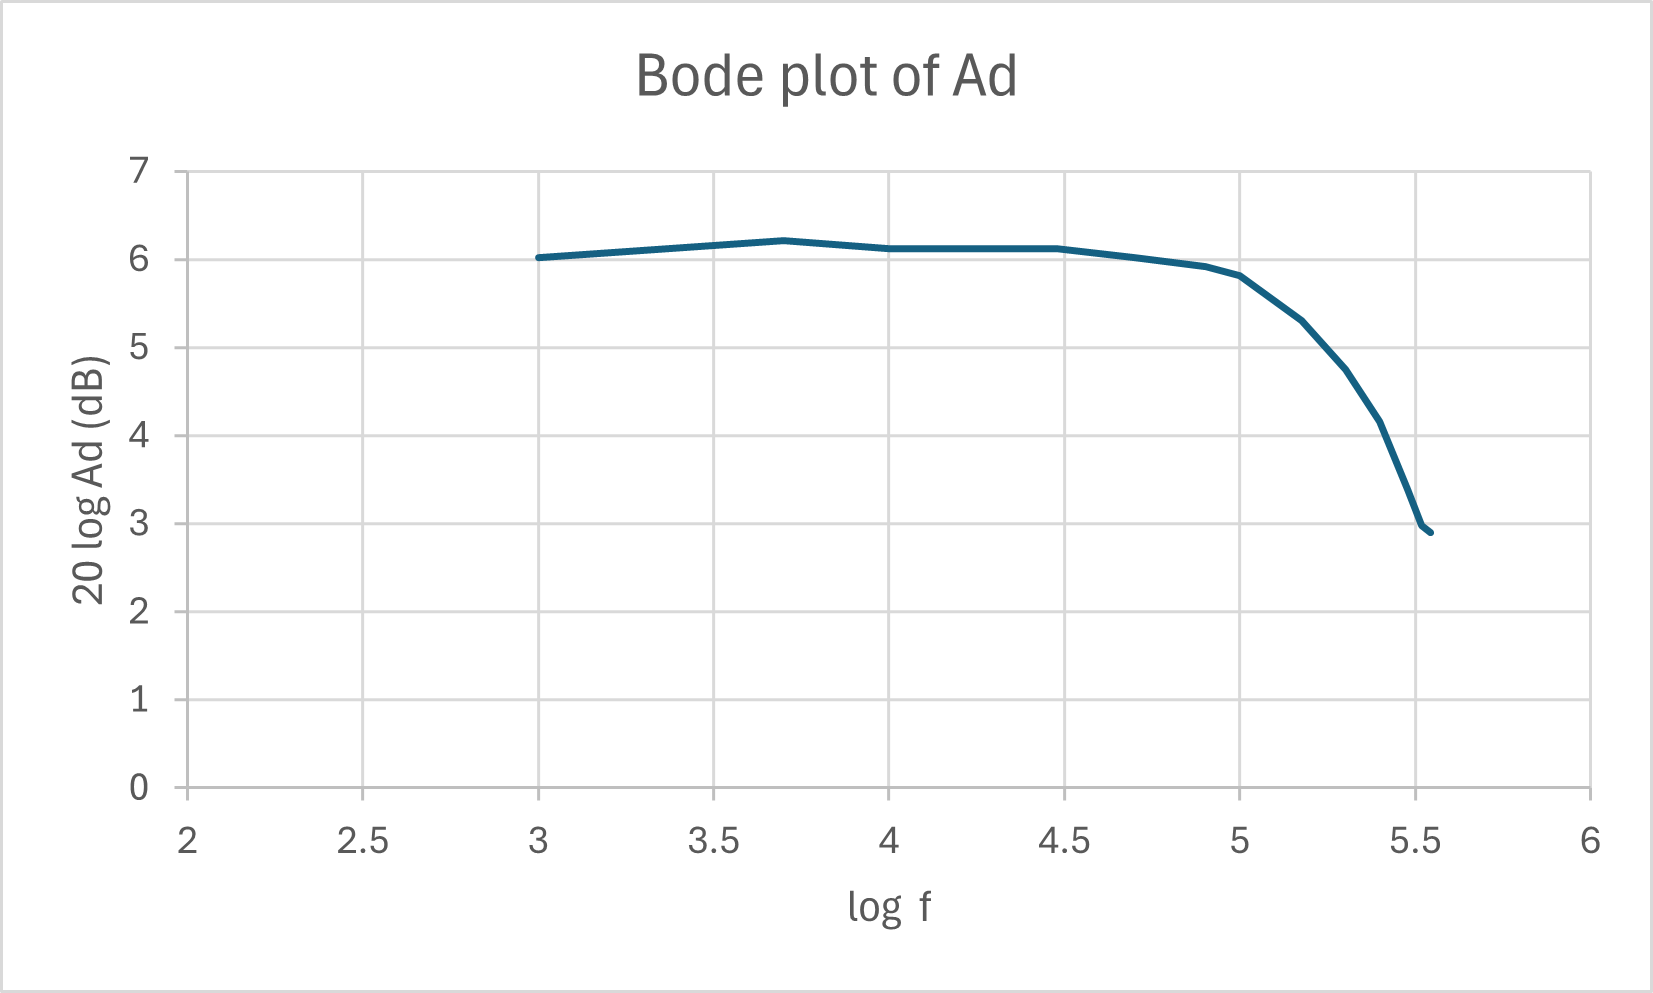
\includegraphics[scale=0.65]{Bode_plot_Ad.png}
        \caption{Bode Plot of $A_{d}$}
    \end{figure}
    \end{minipage}

\end{CJK*}
\end{document}